\documentclass[a4paper,11pt]{article}
\usepackage[utf8]{inputenc}
\usepackage{amsmath}
\usepackage{amsfonts}
\usepackage{amssymb}
\usepackage{graphicx}
\usepackage{braket}

\numberwithin{equation}{section}
\renewcommand\thesubsection{\alph{subsection}}
\newcommand{\bvp}[1]{\mathbf{#1}'}
\newcommand{\bv}[1]{\mathbf{#1}}
\newcommand{\ez}{\epsilon_0}
\newcommand{\eo}{\epsilon_1}
\newcommand{\lrp}[1]{\left({#1}\right)}
\newcommand{\lrb}[1]{\left\{{#1}\right\}}


%opening
\title{Solid State 1 HW2}
\author{Vince Baker, Tony Wang}

\begin{document}
\maketitle

\section*{1}
\begin{figure}[h]
 \caption{Lattice structure}
 \centering
   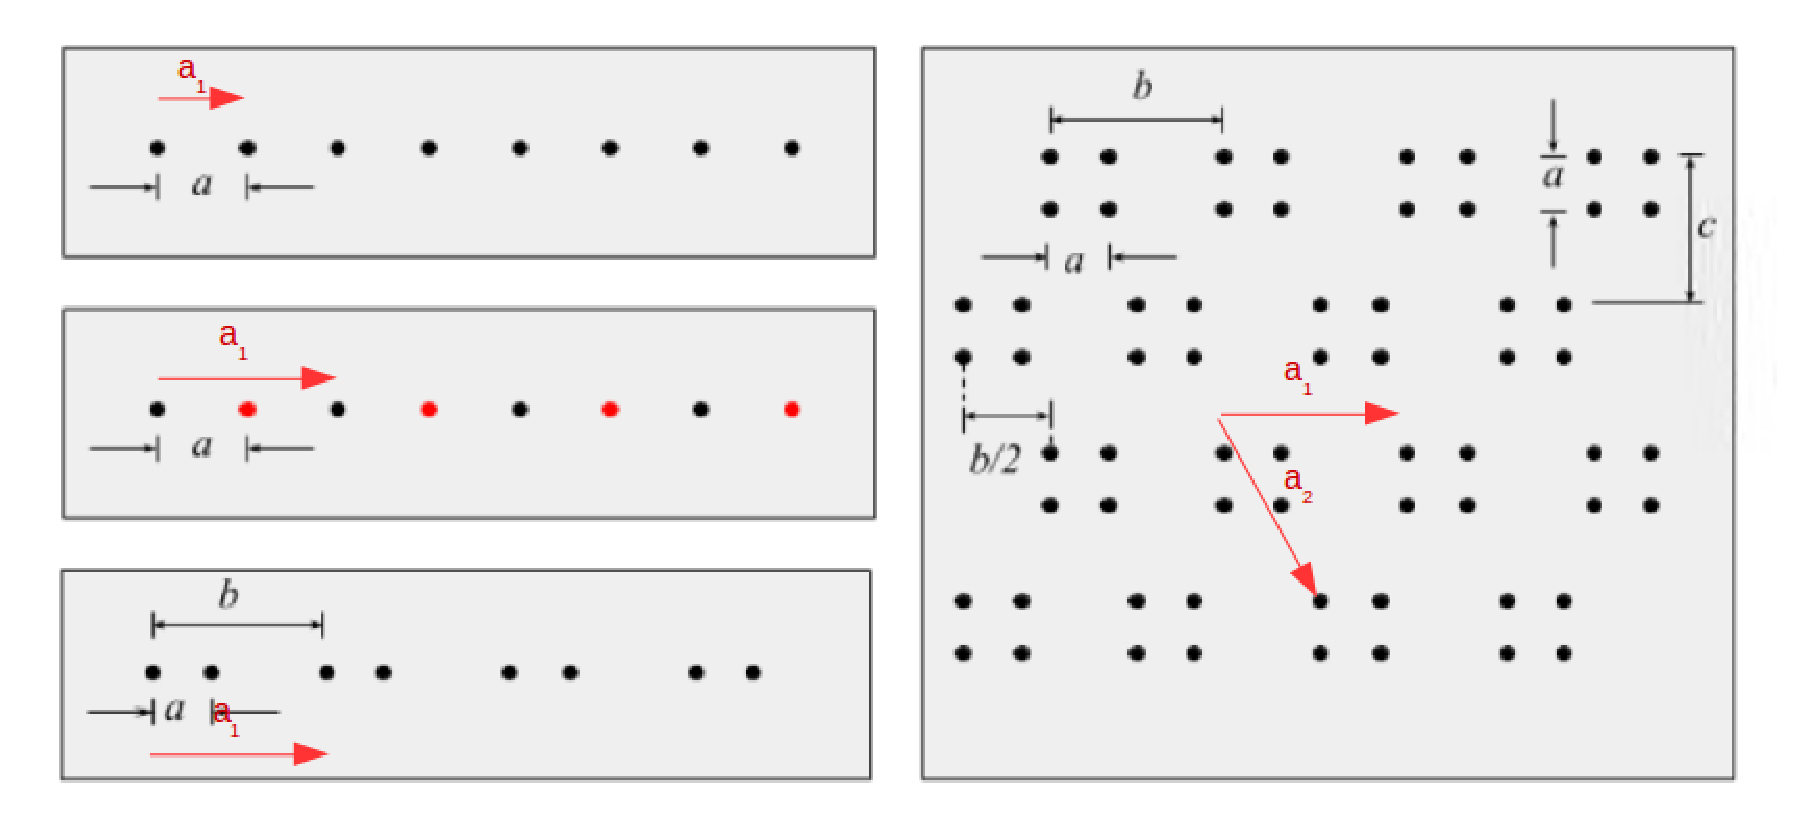
\includegraphics[width=\textwidth]{p1}
\end{figure}
For the first structure, the lattice vector is $\bv{a}_1=a\bv{\hat{x}}$ and the basis is a single molecule.\\
\\
For the second structure, the lattice vector is $\bv{a}_1=2a\bv{\hat{x}}$ and the basis are the two different molecules separated by a.\\
\\
For the third structure, the lattice vector is $\bv{a}_1=b\bv{\hat{x}}$ and the basis is two of the same molecule separated by a.\\
\\
For the fourth structure, the lattice vectors are $\bv{a}_1=b\bv{\hat{x}}, \bv{a}_2=\frac{b}{2}\bv{\hat{x}}+c\bv{\hat{y}} $ and the basis is a square of four molecules of side a.\\
\section*{2}
\begin{figure}[h]
 \caption{Lattice structure}
 \centering
   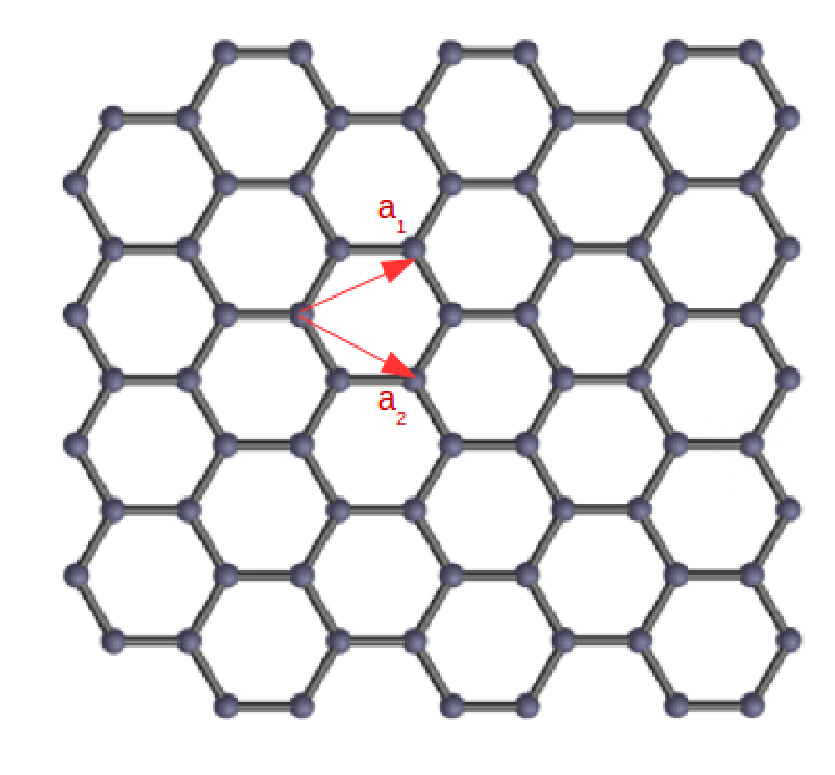
\includegraphics[width=\textwidth]{p2}
\end{figure}
For graphene the primitive cell is a single 6-atom ring. 
One choice of translation vectors that carry one ring into another is $\bv{a}_1=(1+\cos{(60)})\bv{\hat{x}}+\sin{(60)}\bv{\hat{y}}, \bv{a}_2=(1+\cos{(60)}\bv{\hat{x}})-\sin{(60)}\bv{\hat{y}}$ where we take the nearest-neighbor distance as 1. 

\section*{3}
In the hcp structure as given the centers of the spheres are separated by length $a$. 
Assuming the black spheres in the center have the same radius as the white spheres, each black sphere makes a regular tetrahedron of side length $a$ with three of the white spheres in the bottom layer and the top layer.
The height of each tetrahedron is $\frac{\sqrt{6}}{3}a$, so $c=\frac{2\sqrt{6}}{3}a$ and $c/a = \sqrt{8/3}$.\\
\\
To determine the number of nearest neighbors, and hence the coordination number, we examine the white sphere in the center of the bottom layer.
Its nearest neighbors at distance $a$ include the 6 adjacent white spheres, the three black spheres in the center and the three black spheres in the unit cell below.
Therefore the number of nearest neighbors is 12.

\end{document}
